\documentclass[tikz,border=3mm]{standalone}
\usepackage{amsmath,amssymb}
\renewcommand{\familydefault}{\sfdefault}
\usepackage{tikz}
\usepackage{pgfplots}
\pgfplotsset{compat=1.18}
\usetikzlibrary{
  arrows.meta,
  positioning,
  calc,
  fit,
  backgrounds,
  shapes.geometric,
  pgfplots.fillbetween
}

\definecolor{R7Navy}{HTML}{17324D}
\definecolor{R7Teal}{HTML}{0A8F8F}
\definecolor{R7Gold}{HTML}{E0A12B}
\definecolor{R7Coral}{HTML}{D85D55}
\definecolor{R7Violet}{HTML}{6757C7}
\definecolor{R7Sky}{HTML}{5AA6C8}
\definecolor{R7Ink}{HTML}{243746}
\definecolor{R7Muted}{HTML}{667784}
\definecolor{R7Pale}{HTML}{EEF4F5}
\definecolor{R7Warm}{HTML}{FFF6E5}
\definecolor{R7Paper}{HTML}{FCFDFD}

\tikzset{
  r7box/.style={
    rounded corners=2.2mm,
    very thick,
    align=center,
    minimum height=23mm,
    text width=29mm,
    inner sep=3.2mm
  },
  r7arrow/.style={
    -{Stealth[length=2.4mm,width=1.8mm]},
    line width=1.0pt,
    color=R7Muted
  },
  r7tag/.style={
    font=\bfseries\scriptsize,
    text=R7Navy,
    fill=white,
    inner sep=1.2pt
  }
}

\pgfplotsset{
  r7axis/.style={
    axis line style={R7Ink, line width=0.8pt},
    tick style={R7Ink, line width=0.7pt},
    tick label style={font=\footnotesize, text=R7Ink},
    label style={font=\small, text=R7Ink},
    title style={font=\bfseries\small, text=R7Navy, yshift=1mm},
    grid=both,
    major grid style={draw=R7Muted!22, line width=0.45pt},
    minor grid style={draw=R7Muted!10, line width=0.35pt},
    legend style={
      draw=none,
      fill=white,
      fill opacity=0.92,
      text opacity=1,
      font=\scriptsize,
      cells={anchor=west}
    }
  }
}

\begin{document}
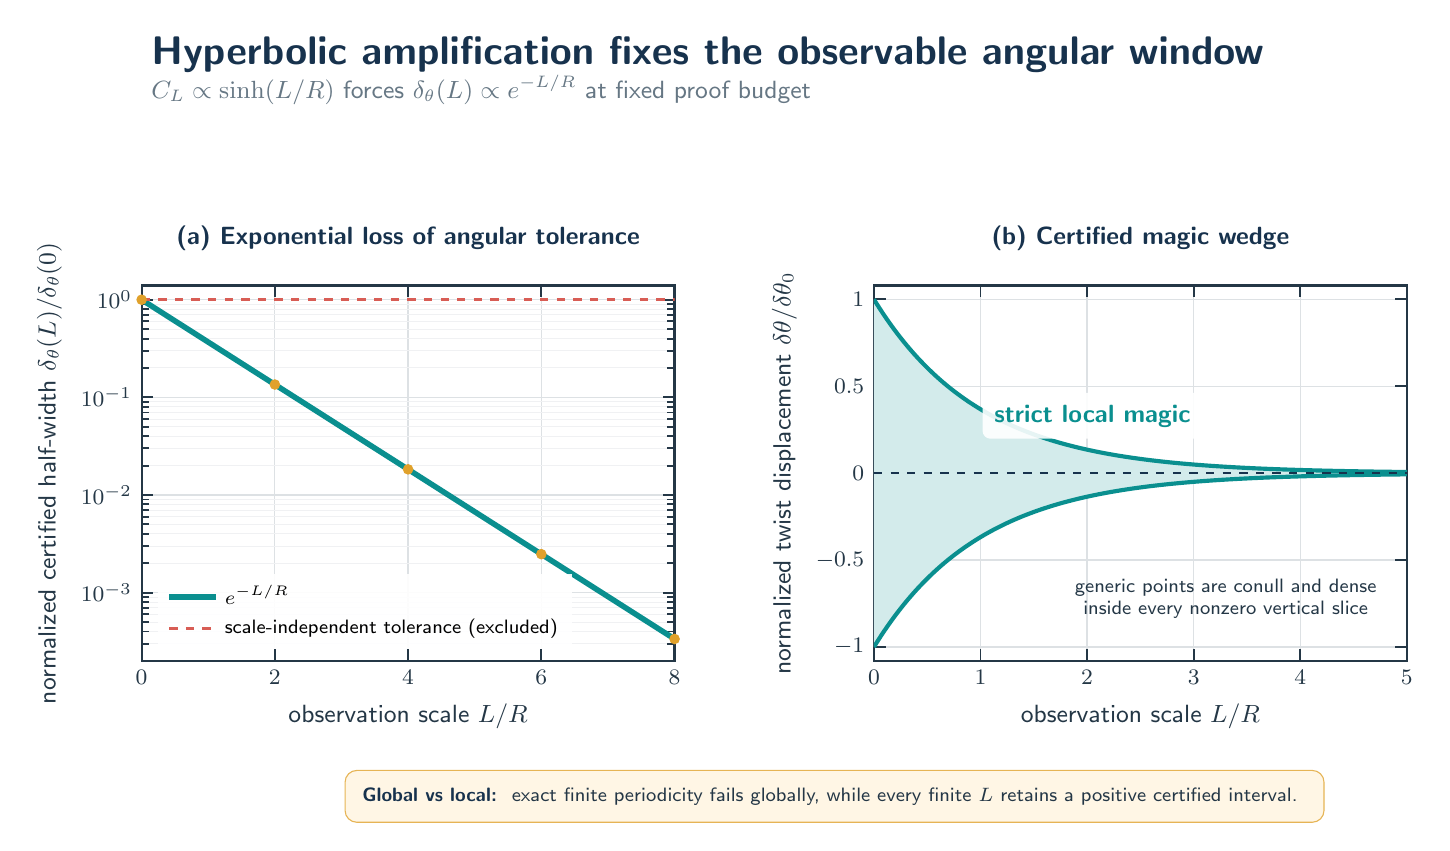
\begin{tikzpicture}[font=\sffamily]
  \node[anchor=west,font=\bfseries\Large,text=R7Navy] at (0,7.7)
    {Hyperbolic amplification fixes the observable angular window};
  \node[anchor=west,font=\small,text=R7Muted] at (0,7.25)
    {$C_L\propto\sinh(L/R)$ forces $\delta_\theta(L)\propto e^{-L/R}$ at fixed proof budget};

  \begin{axis}[
    r7axis,
    at={(0,0)},
    anchor=south west,
    width=8.35cm,
    height=6.35cm,
    ymode=log,
    xmin=0,xmax=8,
    ymin=2e-4,ymax=1.4,
    xlabel={observation scale $L/R$},
    ylabel={normalized certified half-width $\delta_\theta(L)/\delta_\theta(0)$},
    title={(a) Exponential loss of angular tolerance},
    legend pos=south west
  ]
    \addplot[domain=0:8,samples=180,line width=2pt,R7Teal]
      {exp(-x)};
    \addlegendentry{$e^{-L/R}$}
    \addplot[domain=0:8,samples=2,line width=1.1pt,dashed,R7Coral]
      {1};
    \addlegendentry{scale-independent tolerance (excluded)}
    \addplot[only marks,mark=*,mark size=1.7pt,R7Gold]
      coordinates {(0,1)(2,0.135335)(4,0.0183156)(6,0.00247875)(8,0.00033546)};
  \end{axis}

  \begin{axis}[
    r7axis,
    at={(9.3cm,0)},
    anchor=south west,
    width=8.35cm,
    height=6.35cm,
    xmin=0,xmax=5,
    ymin=-1.08,ymax=1.08,
    xlabel={observation scale $L/R$},
    ylabel={normalized twist displacement $\delta\theta/\delta\theta_0$},
    title={(b) Certified magic wedge},
    ytick={-1,-0.5,0,0.5,1},
    legend pos=north east
  ]
    \addplot[name path=upper,domain=0:5,samples=160,draw=R7Teal,line width=1.5pt]
      {exp(-x)};
    \addplot[name path=lower,domain=0:5,samples=160,draw=R7Teal,line width=1.5pt]
      {-exp(-x)};
    \addplot[fill=R7Teal!18,draw=none]
      fill between[of=upper and lower];
    \addplot[domain=0:5,samples=2,dashed,R7Navy,line width=0.9pt] {0};
    \node[font=\bfseries\small,text=R7Teal,fill=white,fill opacity=0.9,
      text opacity=1,rounded corners=1mm,inner sep=1.5mm]
      at (axis cs:2.05,0.33) {strict local magic};
    \node[font=\scriptsize,text=R7Ink,align=center]
      at (axis cs:3.3,-0.72)
      {generic points are conull and dense\\inside every nonzero vertical slice};
  \end{axis}

  \node[rounded corners=1.5mm,draw=R7Gold!80,fill=R7Warm,
    font=\scriptsize,text=R7Ink,align=left,inner sep=2.2mm]
    at (8.8,-1.72) {
      \textbf{\color{R7Navy}Global vs local:}\;
      exact finite periodicity fails globally, while every finite $L$ retains a positive certified interval.
    };
\end{tikzpicture}
\end{document}
